%!TEX root = cvl_bachelor_thesis.tex

%-------------------------------------------------------
% Methodology
%-------------------------------------------------------
\section{Methodology}
\label{sec:methodology}

%----------------------------------------------
% * Verwendetet Technologien
%----------------------------------------------
\subsection{Verwendetet Technologien und Protokolle}
\label{sec:Verwendetet Technologien}
Bevor auf die eigentliche Umsetzung eingegangen wird werden die verwendeten Frameworks und Technologien dargestellt.
Ein Teil davon, wie HTTP und REST, wurden bereits durch das Interface für KRESHMOI festgelegt, 
ein weiterer ergab sich durch die Anforderung einer Web-Applikation.
Die Frameworks und Technologien für Grafik und GUI wurden gewählt weil mit ihnen eine schnelle Umsetzung der Anforderungen möglich war.

%----------------------------------------------
% ** HTTP
%----------------------------------------------
\subsubsection{HTTP}
\label{sec:HTTP}
HTTP (Hyper Text Transfer Protokoll) ist ein Protokoll zur Übertragung von Daten über ein Netzwerk welches auf TCP aufsetzt.
Der Datenaustausch zwischen zwei Kommunikationspartnern findet in der Form von Nachrichten statt, 
wobei der Client eine Anfrage an einen Server stellt und dieser die Anfrage bearbeitet und eine Antwort returniert.
%
Eine Nachricht setzt sich aus einem Header und einen Body zusammen.
Der Body enthält die Nutzdaten und der Header enthält Metadaten über die Nutzdaten.
Vom Aufbau der Nachricht unterscheiden sich Anfrage und Antwort nur in der ersten Zeile:
\begin{itemize}
	\item Anfrage: Enthält die HTTP-Methode, die URL welche auf die Resource am Server zeigt und die Protokollversion.
	\item Antwort: Enthält die Protokollversion und den Serverstatus. 
		Der Serverstatus liefert eine Aussage ob der Request erfolgreich bearbeitet wurde bzw welche Art von Fehler bei der Bearbeitung aufgetreten ist.
\end{itemize}
HTTP ist ein zustandsloses Protokoll, daher wird nach jeder Anfrage die Verbindung vom Server wieder abgebaut.
Für eine Zuordnung eines Clients muss dieser eine Session-ID mitsenden welche normalerweise im Header enthalten ist \cite{http}.

%--------------------------------------------- 
% ** REST
%----------------------------------------------
\subsubsection{REST}
\label{sec:HTTP}
REST ist im eigentlichen Sinn mehr ein Architekturstil als ein Protokoll welcher mit HTTP umgesetzt wird.
Die Idee von REST ist, dass eine URL genau eine Ressource auf einem Server adressiert, 
wobei eine Ressource eine statische Datei oder das Ergebnis einer Aktion auf dem Server sein kann.
Dieser Architekturstil lässt sich durch fünf Prinzipiell zusammenfassen:
\begin{itemize}
	\item \textbf{Ressource mit eindeutiger Identifikation:}
		Jede Ressource wird durch eine URI (Uniform Resouce Identifier) weltweit eindeutig identifiziert.
		Diese adressiert unter anderem den Server auf den sich die Ressource befindet sowie Ressource auf dem Server selbst.
	\item \textbf{Hypermedia:}
		Verknüpfungen zu anderen Entitäten werden als Links auf die jeweiligen Ressourcen dargestellt.
		Weiters kann die Steuerung des Applikationszustandes durch Links auf weiter Aktionen durch Hypermedia umgesetzt werden.
	\item \textbf{Standard-Opperationen:}
		Es gibt ein definiertes Interface welches von jeder Ressource zur Verfügung gestellt werden muss.
		Dieses umfasst einen relativ kleinen Satz von Operationen welche auf die Ressource ausgeführt werden können.
	\item \textbf{Unterschiedliche Repräsentation der Resourcen:}
		Die Ressourcen können unterschiedliche Darstellungsformen haben.
		Ein Client kann also eine Ressource in einem bestimmten Format (z.B.: XML, HTML, JSON) anfordern,
		sofern diese Darstellung vom Server für die jeweilige Ressource unterstützt wird.
		In HTTP wird die gewünschte Darstellung im Header angegeben.
	\item \textbf{Zustandslose Kommunikation}
		Der Server hält keine Zustandsinformationen über den Client welche über die Dauer eines Requests hinaus gehen.
		Daher muss der Zustand einer Anwendung entweder am Client liegen oder vom Server in eine Ressource umgewandelt werden \cite{rest}. 
\end{itemize}


%----------------------------------------------
% ** JSON
%----------------------------------------------
\subsubsection{JSON}
\label{sec:JSON}
Bei JSON (JavaScript Object Notation) handelt es sich um ein Datenformat zum Austausch von Arrays und Objekt-Graphen.
JSON findet neben XML vor allem in der Kommunikation zwischen Client und Server bei Webanwendungen Verwendung, 
wobei JSON Daten wesentlich kompakter und damit ressourcensparender sind.
Wie bei XML werden Listen und Objekte in einer von Menschen lesbaren Form darstellt.
Dabei werden folgende Datentypen unterstützt, welche wiederum beliebig tief ineinander verschachtelt werden können: NULL, Boolean, Zahl, String, Array und Objekt \cite{ajax}.

%----------------------------------------------
% ** AJAX
%----------------------------------------------
\subsubsection{AJAX}
\label{sec:AJAX}
AJAX (Asynchronous JavaScript and XML) ermöglicht es einer Webanwendung,kleinere Mengen von Daten nachzuladen und damit Teile der Webseite dynamisch zu ändern, 
statt bei jeder Aktion die Webseite neu zu laden.
Benötigt die Weapplikation Daten vom Server, wird an diesen eine HTTP Anfrage gesendet und Callback-Funktionen für den Fall einer Antwort oder eines Fehlers beim Browser registriert.
Erhält der Browser eine Antwort auf seine Anfrage ruft er die Callback-Funktion auf und übergibt die erhalten Daten, wodurch die Webanwendung mit der Verarbeitung dieser fortfahren kann.
Dies ermöglicht die Entwicklung komplexer Webapplikationen, 
wobei die Webapplikation selbst mit der Seite geladen wird und die Daten, die der Benutzer mit der Anwendung verarbeiten möchte, dynamisch von der Anwendung nachgeladen werden können \cite{ajax}.

%----------------------------------------------
% ** Objectiv-J
%----------------------------------------------
\subsubsection{Objectiv-J}
\label{sec:Objectiv-J}

Objective-J ist eine Programmiersprache welche sich von der Syntax stark an Objective-C anlehnt.
Sie ist eine Erweiterung oder Obermenge von Javascript und wird von einem in Javascript geschriebenen Interpreter abgearbeitet.
In Javascript können Objekte durch Prototyping erstellt werden, das Konzept von Klassen wird aber nicht unterstützt.
Objective-J bietet zusätzlich zu den nativen JavaScript Objekten die Definition von Klassen inklusive Vererbung und die Generierung von Objekten daraus.
Obwohl es die Sprache erlaubt für Variablen, Methodenparameter und Rückgabe einer Funktion einen Datentyp zu definieren, 
werden diese aufgrund von schwacher Typisierung vom Interpreter nicht auf ihre Einhaltung überprüft.
In der aktuellen Version wird die Übergabe von Referenzen als Parameter ähnlich einem Pointer in C unterstützt \cite{capp}.

%----------------------------------------------
% ** Cappuccino
%----------------------------------------------
\subsubsection{Cappuccino}
\label{sec:Cappuccino}
Bei Cappuccino handelt es sich um ein Web Application Framework für Objectiv-J und JavaScript, welches hauptsächlich der Erstellung komplexer Benutzeroberflächen dient.
Das Framework lehnt sich sowohl vom Aussehen als auch von der Benennung der Komponenten sehr stark an das GUI-Framework Cocoa von Apple an.
GUI-Elemente werden als Objekte erstellt welche von einer View-Klasse erben und innerhalb von anderen Views positioniert werden können.
Das Interface wird von einem HTML-fähigen Browser gerendert, 
\C{wobei durch die Abstraktion durch die Komponenten des Frades Frameworks meworks für die Entwicklung keinerlei HTML oder CSS Kenntnisse notwendig sind}\cite{capp}.


%----------------------------------------------
% ** WebGL 
%----------------------------------------------
\subsubsection{WebGL}
\label{sec:WebGL}
WebGL ist eine API für die Erstellung von 2D und 3D Grafiken in Browsern mit der Unterstützung der Grafikkarte.
Im Gegensatz zur Canvas-2D API wo die Bilder in der CPU gerendert werden, ist WebGL aufgrund der Hardwarebeschleunigung wesentlich performanter.
WebGL ist eine shaderbasierte API welche sich sehr stark an OpenGL ES anlehnt.
Dies bedeutet, dass Code für die Shadereinheiten der Grafikpipeline \ref{fig:webgl_graphics_pipeline} entwickelt wird,
welchen der Treiber der Karte in Bytecode übersetzt und zur Ausführung in den Grafikchip lädt.
Die Shaderprogramme werden in der Programmiersprache GLSL geschrieben, welche sich sehr stark an C orientiert.
Der Zugriff auf die Schnittstelle erfolgt über das HTML Canvas Element in welchem die Ausgabe der Grafikkarte dargestellt wird.
Dies geschieht mittels JavaScript, wo die API Funktionen zur Übergabe der Nutzdaten, Befehle und der Shaderprogramme bereitstellt\Rc{das ist kein satz} \cite{webgl-14}.
%TODO: Rene fragen warum dass kein satz ist
\begin{figure}[t]
	\centering
	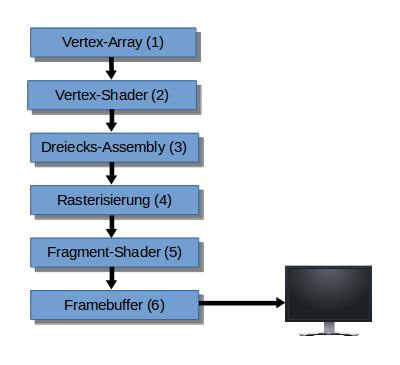
\includegraphics[width=5.2cm]{img/graphics_pipeline.jpg}
	\caption{WebGL Graphik Pipeline}
	\label{fig:webgl_graphics_pipeline}
\end{figure}

Zum Rendern einer Grafik mit der WebGL Grafik Pipeline werden Arrays von Punkten, welche meist die Ecken eines Dreiecks bilden, in einen Vektorbuffer geschrieben.
Diese werden anschließend vom Vertex-Shader verarbeitet, welcher zum Beispiel Skalierung, Rotation oder Transformation auf die Geometrien anwendet oder Farbinfomation hinzufügt.
Anschließend werden aus den Punkten Dreiecke generiert und in der Rasterisierung die Pixel der Dreiecke berechnet.
Die Pixel bekommen dann vom Fragment-Shader ihre Farbe, welcher diese aus Farbinformationen oder aus zuvor übergebenen Textur-Daten generiert.
Nach der Durchführung eines Tiefentests, 
in welchen überprüft wird welche Pixel sichtbar sind und welche von anderen verdeckt werden bzw der Mischung der Farben bei Transparenz, 
werden die Bildinformationen in den Framebuffer geschrieben,
von wo aus Sie auf dem Bildschirm angezeigt werden können \cite{webgl-introduction}.


%----------------------------------------------
% ** PixiJS 
%----------------------------------------------
\subsubsection{PixiJS}
\label{sec:PixiJS}
Da WebGL eine relativ Hardware nahe API ist wurden einige Frameworks entwickelt welche von der Komplexität einer solchen API abstrahieren, zu denen auch PixiJS zählt.
Es bietet Funktionen zum Zeichen von geometrischen Figuren, Füllen von diesen und Laden von Texturen.
Eine Szene in PixiJS ist als Baum organisiert, wobei jeder Knoten in dem Baum wiederum Operationen zur Manipulation wie Transformation, Translation oder Transparenz anbietet.
Ein weiteres Feature ist, dass auf einen Knoten ein Filter mit WebGL Fragment-Shader-Code gesetzt werden kann, welcher zur Manipulation der Farbinformation in den einzelnen Bildpunkte dient \cite{pixijs}.

%----------------------------------------------
% * Funktionalität und Aufbau der Benutzeroberfläche
%----------------------------------------------
\subsection{Funktionalität und Aufbau der Benutzeroberfläche}
\label{sec:Funktionalität und Aufbau der Benutzeroberfläche}
Der Workflow beim Durchsuchen von radiologischen Aufnahmen mit KRESHMOI gliedert sich in folgende Schritte:
\begin{enumerate}
	\item Auswahl eines Start-Datensatzes.
	\item Betrachten des Datensatzes inklusive Fenstern und Zoomen.
	\item Anotieren einer oder mehrerer ROI(s) und eventuelle Eingabe von Text in die Suchzeile.
	\item Suche absenden und Ergebnisse listen.
	\item Betrachen von Datensätzen aus der Ergebnisliste.
	\item Um neue Suchanfrage von ein Ergebnissdatensatz aus zu stellen werden die Schritte von 3 an wiederholt.
\end{enumerate}
Entsprechend dieses Ablaufs wird beim Start der Applikation eine Liste mit allen Datensätzen geladen, 
aus welchen einer als Einstiegspunkt in die Suche ausgewählt werden kann.
Dieser Datensatz wird in den Betrachter der Haupansicht \ref{fig:omip_aplication_layout} geladen.
Die Haupansicht setzt sich aus verschiedenen Interaktions-Elementen (Views) zusammen,
welchen in mehreren möglichen Layouts mit unterschiedlicher Multiplizität und Anordnung miteinander kombiniert werden.
Von diesen Elementen gibt es Vier verschiedene Typen:
\begin{itemize}
	\item Betrachtungsansicht für Volumes (2D-Betrachter)
	\item Betrachtungsansicht für den Report (Report-Betrachter)
	\item Präsentationsansicht für die Ergebnisse (Ergebnis-Liste)
	\item Eingabezeile für Schlagwörter mit dem Suchbutton (Suchzeile)
\end{itemize}
Die Fläche welchen die einzelnen Views innerhalb des Browserfensters einnehmen kann zwischen den Views beliebig verschoben werden, 
unter der Prämisse dass die Bedienelemente der einzelnen Views genügend Platz haben.
Auf den Funktionsumfang des 2D-Betrachters und der Ergebnis-Liste wird in den folgenden Unterkapiteln etwas genauer eingegangen.
\begin{figure}[t]
	\centering
		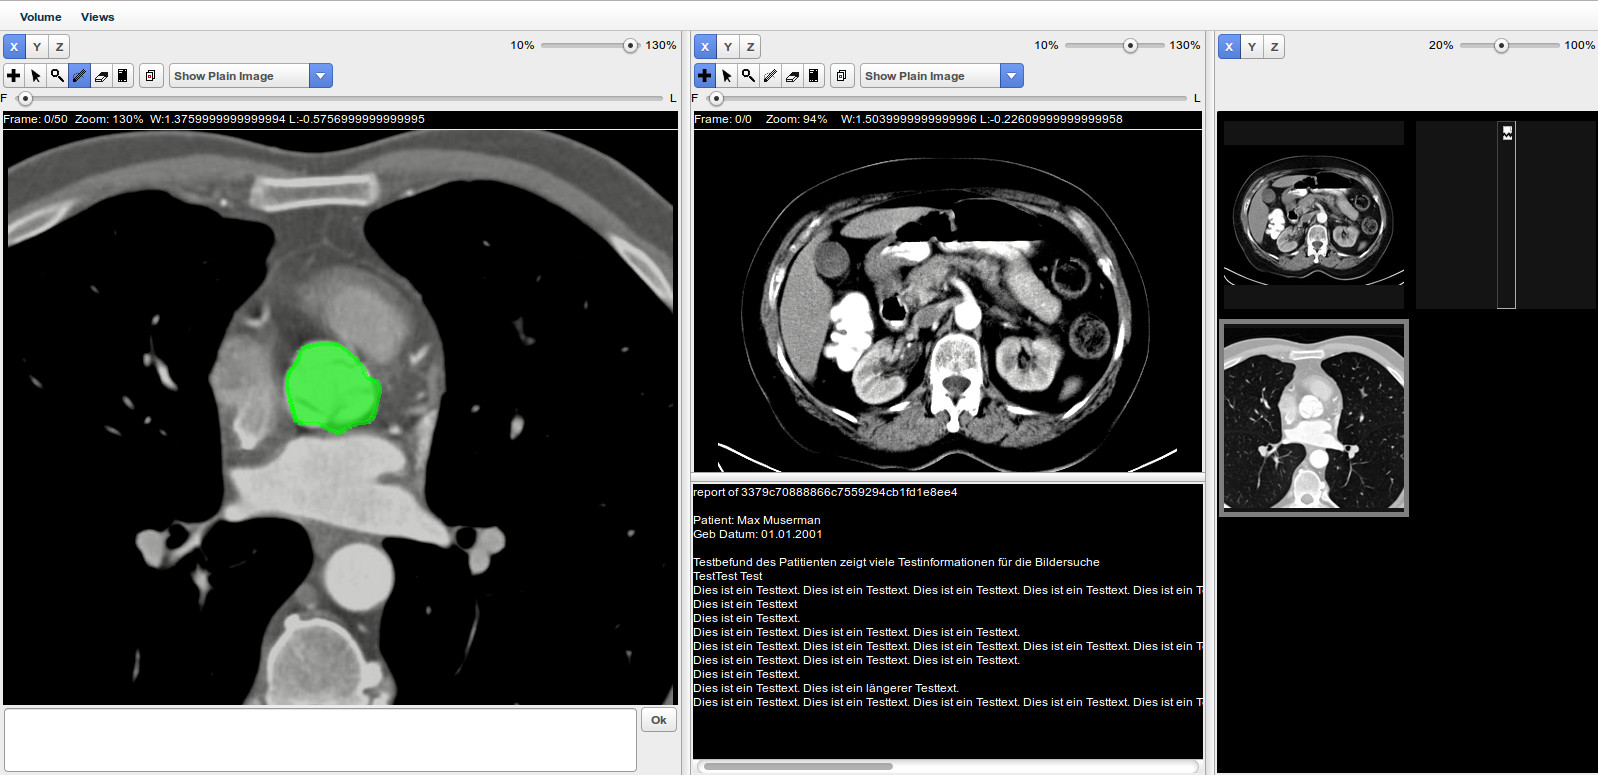
\includegraphics[width=0.8\linewidth]{img/c3_application_standard.jpg}
	\caption{Hauptansicht mit Layout für zwei 2D-Betrachter, Report-Betrachter und Ergebnis-Liste}
	\label{fig:omip_aplication_layout}
\end{figure}


%----------------------------------------------
% ** Funktionalität des 2D-Betrachters
%----------------------------------------------
\subsubsection{Funktionalität des 2D-Betrachters}
\label{sec:Funktionalität des 2D-Betrachters}
Der 2D-Betrachter orientiert sich von seinen Funktionen sehr stark an der Betrachtungssoftware einer PACS-Workstaion oder eines DICOM-Betrachters.
Er ermöglicht die räumliche Navigation durch die Schnitte eines Volumes in einer bestimmten Orientierung, sowie das Umschalten zwischen den Orientierungen.
Des weiteren kann wenn das Volume aus der Ergebnissliste einer Suche ausgewählt wurde, 
also nicht der Startdatensatz ist,
eine Anzeige mit den Deckungsbereichen der Suche hinzu geschaltet werden. 

Zur Interaktion mit den Volume wird auch wie bei anderen Betrachtern der Maus eine bestimmte Funktion zugewiesen.
Die Funktionen umfassen Fensterung, Zoom, Bewegen des Bildes und Zeichnen und Löschen von Polygonen (ROIs).
Das Einzeichnen von ROIs ist um die Benutzung einfach zu halten auf ein einzelnes Schnittbild beschränkt.
Wird das Werkzeug zum Zeichen oder Löschen von Polygonen auf mehreren Schnitten verwendet springt der Betrachte bei deren Aktivierung immer wieder auf das Schnittbild mit dem ersten Polygon zurück.
Das Bild kann halb Transparent mit dem Report des Datensatzes überblendet werden, was aber die Mausfunktion auf das Scrollen des Reports reduziert.
In allen anderen Funktionen ist das Scrollen immer an die Navigation durch die Schnitte gebunden.

%----------------------------------------------
% ** Funktionalität der Ergebniss-Liste
%----------------------------------------------
\subsubsection{Funktionalität der Ergebniss-Liste}
\label{sec:Funktionalität der Ergebniss-Liste}
Die Ergebnis-Liste präsentiert die Ergebnisse einer Suche welches sie über Drag and Drop in einen Betrachter laden lassen.
Die Präsentation erfolgt über ein Vorschaubild welches von KRESHMOI als repräsentatives Bild für die Suche gewählt wurde.
Um ein Suchergebniss im Vorfeld zu Beurteilen verfügt die Ergebnis-List ebenfalls über die Funktion die Orientierung der Schnitte des Volumes zu ändern und die Vorschaubilder zu zoomen.

%----------------------------------------------
% * Technische Umsetzung
%----------------------------------------------
\subsection{Technische Umsetzung}
\label{sec:Technische Umsetzung}
In dem Unterkapitel Technische Umsetzung wird im Groben die Archtiktur der Applikation sowie von komplexeren Komponenten erklärt und auf wichtige Details bei deren Umsetzung eingegangen.
Weiters wird angegeben wie die Fensterung mit zwei verschidenen Technologie implementiert wurde.

%----------------------------------------------
% ** Umsetzung der dynamischen Layouts
%----------------------------------------------
\subsubsection{Framework für dynamischen Layouts}
\label{sec:Umsetzung der dynamischen Layouts}

%----------------------------------------------
% ** Berehnung der Fensterung
%----------------------------------------------
\subsubsection{Berechnung der Fensterung}
\label{sec:Berehnung der Fensterung}
Die Berechnung der Fensterung ist eine Anpassung von Kontrast und Helligkeit des Bildes,
wozu für jedes Pixel der Farbwert mit einer Linear Transformation in einen neuen Zielwert überführt werden muss.
\begin{equation}
        F(x) = c*x + b
\end{equation}
Dabei ist der Kontrast durch $c$ und die Helligkeit durch $b$ gegeben.
Für diese Berechnung wurde ein Ansatz auf Basis von JavaScript durch die Canvas 2D API und eine Implementierung mit Web GL getestet.

\paragraph{Canvas 2D API}
Für die graphische Ausgabe im Browser wird ein HTML5 Canvas Element verwendet,
auf welches über ein sogenanten Grafikkontext zugegriffen werden kann. 
Dieser Grafikkontext wird in JavaScript vom Browser als Objekt zur Verfügung gestellt.
Durch das Kontext-Objekt kann der Bildinhalt in ein Array von Farbwerten und umgekehrt auch ein Array von Farbwerten in das Bild geschrieben werden.
Dabei wird das Bild zeilenweise in ein eindimensionales Array Serialisiert, 
wo jeder Bildpunkt auf 4 Speicherstellen mit einem Integer-Wert zwischen 0 und 255 abgebildet wird.
Die ersten drei Speicherstellen bilden den Farbwert durch die Anteile von Rot, Grün, Blau und die vierte den Alpha Kanal.
Für die Fensterung müssen alle Speicherstellen für die Farbe transformiert und wieder auf einen Integer Wert gerundet werden.
%
Um unnötige Berechnungen für jedes einzelne Pixel zu sparen, werden pro Fensterungsschritt alle Pixelwerte zwischen 0 und 255 einmal vor berechnet und in einer LookUp Tabelle als Array gespeichert.
Anstatt den Wert für jedes Pixel neu zu berechen und zu runden fungiert bei diesem Ansatz der aktuelle Wert eines Pixels als Schlüssel für die Tabelle welche den neuen Wert des Pixels enthält.
Die Anzahl der Operationen wird dabei auf 255 Berechnungen und die Anzahl der Speicherzugriffe pro Bildpunkt sowie die der LookUp Tabelle reduziert.
\begin{figure}[t]
\begin{lstlisting}[
	language=JavaScript,
	firstnumber=1,
	caption=Ändern von Kontrast und Helligkeit in einem HTML Canvas Element mit einer LookUp Tabelle in JavaScript
]
function calcWindowForDomElement(domElement, contrast, brightness)
{
    var ctx = domElement.getContext("2d");
    var w = domElement.width;
    var h = domElement.height;

    var lut = getLookUpTable(contrast, brightness);
    var image = ctx.getImageData(0, 0, w, h);
    var imageData = image.data;
    var imageDataSize = (w * h * 4);

    for(var pos = 0; pos < imageDataSize; pos = pos + 4){
        imageData[pos] = lut[imageData[pos]];
        imageData[pos + 1] = lut[imageData[pos + 1]];
        imageData[pos + 2] = lut[imageData[pos + 2]];
    }

    ctx.putImageData(image,0,0);
}
\end{lstlisting}
\end{figure}
%
\begin{figure}[t]
\begin{lstlisting}[
	language=JavaScript,
	firstnumber=1,
	caption=Berechnung der LookUp Tabelle
]
function getLookUpTable(contrast, brightness){
    var lut = new Array();

    for(var i = 0; i < 256; i++){
        var newVal = Math.round(contrast * i + brightness);
        if(newVal < 0) newVal = 0;
        if(newVal > 255) newVal = 255;
        lut[i] = newVal;
    }

    return lut;
}
\end{lstlisting}
\end{figure}

\paragraph{WebGL}
Die Berechnung der Fensterung in der WebGL Grafik Pipeline erfolgt im Fragment-Shader.
Dazu wird über die WebGL-API zuerst ein Array von Punkten, 
welches die Grundfläche in der Form von zwei aneinander liegenden Dreiecken darstellt übergeben.
Weiters wird das Bild für die Fensterung als Textur in den Speicher der Grafikkarte geladen und die Variablen für Helligkeit und Kontrast übergeben.
Der Vertex-Shader fügt den Punkten einen Vektor mit Textur-Koordinaten hinzu, welche an den Fragment-Shader weitergereicht werden.
Dieser kann dann mit Hilfe der Textur-Koordinaten für jedes Pixel der Grundfläche die Farbe des Pixels aus der gepufferten Textur laden.
Die Repräsentation der Farbe erfolgt mit dem Datentyp $vec4$ welcher eine Vierdimensionalen Vektor für Fließkommazahlen darstellt.
Die ersten Drei Dimensionen bilden die Drei Grundfarbe Rot, Grün, Blau die vierte den Alpha-Kanal, welche jeweils von einem Wert zwischen 0 und 1 repräsentiert werden.
Bevor die Farb-Information des Pixels zurückgegeben wird erfolgt die Fensterung durch einen Linear-Transformation auf die drei Farbkanäle des Farbvektors.
Die Rückgabe der Farbinformation erfolgt durch das ablegen in der Variable $gl\_FragColor$.
\begin{figure}[t]
\begin{lstlisting}[
	language=GLSL,
	firstnumber=1,
]
precision mediump float;

uniform sampler2D u_image;
varying vec2 vTextureCoord;

uniform float contrast;
uniform float brightness;

void main() {
    vec4 color = texture2D(u_image, vTextureCoord);
    gl_FragColor.r = color.r * contrast + brightness;
    gl_FragColor.g = color.g * contrast + brightness;
    gl_FragColor.b = color.b * contrast + brightness;
    gl_FragColor.a = color.a;
}
\end{lstlisting}
\caption{Fragment-Shader-Code zum Rendern und Fenstern der Slices}
\end{figure}


%----------------------------------------------
% ** 2D Betrachter
%----------------------------------------------
\subsubsection{2D Betrachter}
\label{sec:2D Betrachter}
Für die Implementierung des 2D-Betrachters wurde neben Cappuccino für die Bedienelemente auch noch Pixi.JS für das Grafikfenster zur Darstellung des Volumes verwendet.
Der Inhalt des Grafikfensters ergibt sich aus den inhalt von mehreren übereinanderliegenden Layern.
\begin{itemize}
	\item \textbf{ImageLayer} zur Darstellung der Schnitte des Volumes
	\item \textbf{AnotationLayer} zum zeichnen der ROIs
	\item \textbf{ZoomLayer} zur Darstellung des Zoom-Rechecks
	\item \textbf{ReportLayer} zum Render des Berichtes in das Bild
\end{itemize}
Bei diesen Layern werden Skalierung und Positionierung nur auf den ImageLayer und den AnotationLayer angewendet, die anderen füllen jeweils nur das ganze Grafikfenster aus.
Um die Software möglichst erweiterbar zu gestalten,
wurde eine LayerKlasse $PixiLayer$ entwickelt welcher eine beliebige Menge von Sublayern hizugefügt werden kann.
Dabei wird zwischen statischen Sublayern welche jeweils nur die Anzeigefläche ausfüllen und dynamischen Sublayern welche gemeinsam skaliert und positioniert werden können unterschieden.
Diese Layerklasse erledigt auch die konvertierung von Punkten zwischen den dynamischen und den statischen Sublayern, in Hisicht auf Postion, Skalierung und Layerdimension.
Da die restliche GUI mit Cappuccino aufgebaut wurde und dieses Framework auch die Ereignisse für Größenänderungen der einzelen Views behandelt,
müssen diese vom ViewObjekt welches den 2D-Betrachter Kapselt an das Grafikfenster weiter gegeben werden.
Ansonsten ist das Pixi.JS basierte Grafikfenster durch die LayerKlassen bis auf Funktionen zur Übergabe der Anzeigedaten und zur Punktkonvertierung vom 2D-Betrachter abgeschottet.
Die eigentliche Logik des Betrachters ist in den Layern zugeordnete Controller-Klassen gekapselt.
Die Betrachter-Klasse selbst ist hauptsächlich für die Erstelltung der Bedienelemente und die Behandlung von Events verantwortlich.
\begin{figure}[t]
	\centering
		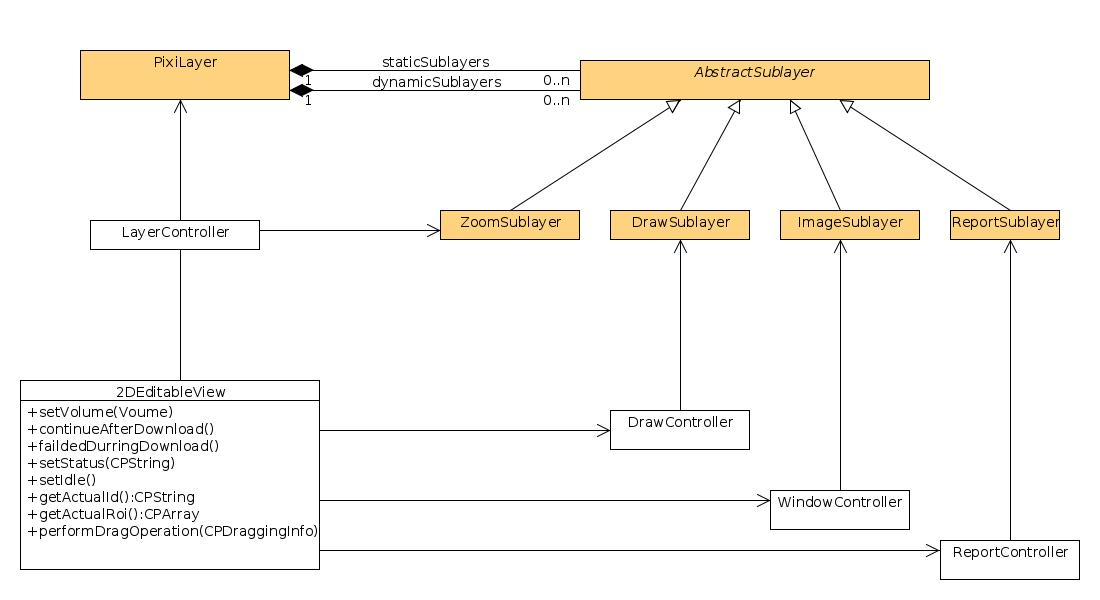
\includegraphics[width=\linewidth]{img/s3_2dview_class_structure.jpg}
	\caption{Struktur des 2D-Betrachters als Klassendiagramm}
	\label{fig:omip_aplication_layout}
\end{figure}

%----------------------------------------------
% * Kommunikation mit KRESHMOI
%----------------------------------------------
\subsection{Kommunikation mit KRESHMOI}
\label{sec:Kommunikation mit KRESHMOI}
Der Datenaustausch mit KRESHMOI basiert auf REST wobei sowohl auf die einzelnen Slices von einem Volume, als auch auf die Suche als Ressource über eine URL zugegriffen werden kann.

%----------------------------------------------
% ** Query nach Bilderns
%----------------------------------------------
\subsubsection{Query nach Bildern}
\label{sec:Query nach Bildern}
Der Zugriff auf die Suchfunktion erfolgt über eine POST-Operation in welcher die Anfrage und die Antwort in JSON codiert werden.
Zum Ausführen einer Suchanfrage stehen zwei Ressourcen zur Verfügung:
\\
\\
\textit{/index}\\
Liefert ein Array von allen Verfügbaren Datensätzen zurück 
\\
\\
\textit{/query}\\
Liefert ein Array von Datensätzen zurück welche anhand der Übergebenen Suchkriterien gefunden wurden.
Eine Suchanfrage basiert immer auf einen Datensatz welcher in der Anfrage übergeben werden muss.
In diesem Datensatz werden weiters Interessante Bereiche sogenannte ROIs (Region of Interesst) in den einzelnen Schnittbildern definiert.
Die Übergabe einer ROI erfolgt als Polygon in Form einer Listen von Punkten im Dreidimensionalen Raum des Volumes.
\begin{figure}[t]
\begin{lstlisting}[
	language=json,
	firstnumber=1,
	caption=Query
]
{
   "queryid":"",
   "text":"",
   "imageid":"",
   "roi": 
   [
      "polygon":
      [
         "point":{"x":0, "y":1, "z":0},
         "point":{"x":1, "y":1, "z":0},
         "point":{"x":0, "y":0, "z":0}
      ],

   ]
}
\end{lstlisting}
\end{figure}


\begin{figure}[t]
\begin{lstlisting}[
	language=json,
	firstnumber=1,
	caption=Result
]
{
   "rankedImageID": 
   [
      {
         "imageID": "9587336b132b127b936ad0afd80ca862",
         "normalDimX": 52,
         "normalDimY": 512,
         "normalDimZ": 512,
         "relevance": 1,
         "report": "",
         "title": "Some Image"
      },
   ]
}
\end{lstlisting}
\end{figure}

%----------------------------------------------
% ** Laden der Bilder
%----------------------------------------------
\subsubsection{Laden der Bilder}
\label{sec:Laden der Bilder}
Die Bilddaten eines Volumes können über eine GET-Operation geladen werden.
Dabei wird jedes Volume als eine Resource im Unterverzeichnis \textit{/image/} identifiziert.
Über Parameter in der URL werden die Schnittrichtung und und die Nummer des Bildes in der jeweiligen Schnittebene angegeben.
Wir keine Nummer für das Bild angegeben wählt KRESHMOI eine repräsentatives Bild für die Suchanfrage, welches für die Präsentation der Ergebnisse verwendet wird.
Für die Schnittebene gibt es entsprechende der Terminologie für die Bildgebung in der Anatomie die Optionen:
\begin{itemize}
	\item Axial: Die Schnitte erfolgen Waagrecht in der Transversalebene
	\item Sagital: Die Schnitte erfolgen Senkrecht in der Sagitalebene
	\item Coronal: Die Schnitte erfolgen Senkrecht in der Frontalebene 
\end{itemize}
Sollen die Regionen welche der Suchanfrage entsprechen in den einzelnen Bildern markiert werden, muss die Query-ID mit übergeben werden um die ursprüngliche Suchanfrage zu identifizieren.
\\
\\
Beispiel:
\\
\url{/image/9587336b132b127b936ad0afd80ca86.jpg?slice=1&direction=axial&query=1}
%TODO: Prüfen ob URL ok
%TODO: Zitieren von KRESHMOI API
%TODO: Zitieren der Schnittebenen
%TODO: Bild ist wikipedia ok: http://de.wikipedia.org/wiki/Anatomische_Lage-_und_Richtungsbezeichnungen
